% Note that the text in the [] brackets is the one that will
% appear in the table of contents, whilst the text in the {}
% brackets will appear in the main thesis.

%% CHAPTER HEADER /////////////////////////////////////////////////////////////////////////////////////
\chapter[Numerical simulation of the GW in the \ac{hsc}]{Numerical simulation of the GW in the \ac{hsc}}
\label{ch:simulation}

%% CHAPTER INTRODUCTION ///////////////////////////////////////////////////////////////////////////////
This chapter presents the sample configuration for numerical simulations based on the \ac{sem}.
The configuration is consistent with the specimen held for experimental validation of the model.
The description includes the overall dimensions of the \ac{hsc} panel, sensor placement, the materials properties, and the excitation signal.
It is shown how the individual components were meshed to optimise computer operations.
In the chapter, two disbonds models are presented; in the first model, the core cells were removed from the damaged area, and in the second model, the interface elements were removed.
%% INCLUDE SECTIONS ///////////////////////////////////////////////////////////////////////////////////

%% SECTION HEADER /////////////////////////////////////////////////////////////////////////////////////
\section{Sample configuration}
\label{sec:sample}

%% SECTION CONTENT ////////////////////////////////////////////////////////////////////////////////////
The sample of interest was a \numproduct{500 x 500 x 1.5} \unit{\cubic\mm} unidirectional \ac{cfrp} plate with stack sequence \(\left[\ang{0},\,\ang{90}\right]_s\) bonded to an aluminium honeycomb core. The volume fraction of fibres was assumed 47\%.
It was decided to use only one skin, as it is pictured in Fig.~\ref{fig:honeycomb}(b), with the intention of experimental validation and to be able to enlarge disbonds between the skin and the core located in the middle of the \ac{hsc} with a tool in a real sample. 
It was not decided to dedicate separate samples for each size of damage because too many factors would affect the signal value, including skin and sensors properties, the thickness of the adhesive layers, position of the core relative to the sensors, and distance between sensor.
Moreover, it renders closely the realistic scenario of monitoring the same structure.
\begin{figure}[H]
	\begin{center}
		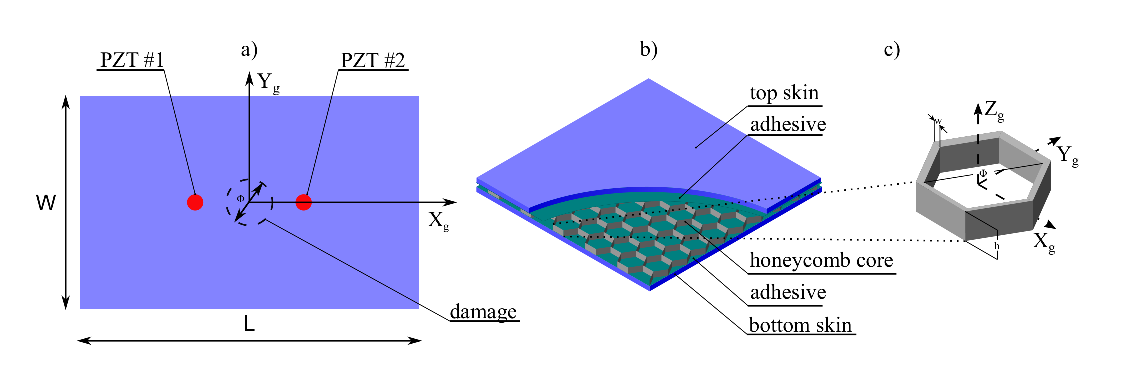
\includegraphics[width=0.95\textwidth]{Chapter_5/honeycomb}
	\end{center}
	\caption{Sample configuration: (\textbf{a}) top view of the sample, (\textbf{b}) \acf{hsc} and (\textbf{c}) details of the honeycomb cell.}
	\label{fig:honeycomb}
\end{figure}

The core geometry is accurately reproduced from the actual specimen, i.e., geometry of irregular hexagonal cells \(\left(\mathrm{h}_1 \ne \mathrm{l}_1\right)\) and double walls at the sheet joints, resulting from the core fabrication technology.
According to the drawing in Fig.~\ref{fig:honeycomb}(\textbf{c}), the cell dimensions are \(\mathrm{w}_c\)=0.1 \unit{\mm}, h\(_1\)=11 \unit{\mm}, h\(_2\)=5 \unit{\mm}, l\(_1\)=10.4 \unit{\mm}, l\(_2\)=6 \unit{\mm} and the cell height g=14.5 \unit{\mm}.
The core was bonded to one \ac{cfrp} plate using the epoxy adhesive (Loctite EA3479B) with the thickness h\(_a\)=0.3 \unit{\mm}.
The adhesive layer covered the entire bottom surface of the skin.

Signal excitation and recording were accomplished with a pair of \acp{pzt}  (Noliac, NCE51) mounted to the top surface of the skin with cyanoacrylate glue.
The circular transducers of diameter \(\Phi_{PZT}\)=10 \unit{\mm} and thickness h\(_{PZT}\)=0.5 \unit{\mm} were attached 200 \unit{\mm} apart, as shown in Fig.~\ref{fig:honeycomb}(\textbf{a}).
The thickness of cyanoacrylate glue under \ac{pzt} was assumed to be h\(_g=50\) \unit{\micro\m}.

The material properties of the components assumed for the simulations are compiled in Tab.~\ref{tab:properties}.
The effective properties of the \ac{cfrp} skin were determined according to the rule of mixtures presented in the book by Vinson and Sierakowski \cite{vinson1993behavior}.
The authors provide a complete description of the homogenisation of composite properties.
Firstly, the stiffness matrix is determined for the single ply of the laminate along the fibre direction.
Then, the stiffness matrix is transformed for other orientations of the laminate plies by the transformation matrix composed of the direction cosines.
In the sample analysed, there are the plies with an orientation of \ang{0} and \ang{90}.
Finally, all the plies in the laminate are homogenised through the thickness.
Explicit expressions of the stiffness components for the laminate modelled by solid elements are presented by Sun and Li in \cite{sun1988three}.
The comprehensive equations to derive the effective stiffness matrix are given in App.~\ref{app:eff_properties} and the resulting \ac{cfrp} properties are shown in Tab.~\ref{tab:properties_eff}.
\begin{table}[H]
	\centering
	\small
	\tabcolsep=0.25cm
	\caption{\label{tab:properties_eff} The effective mechanical properties of the \ac{cfrp} plate and the aluminium honeycomb core for +20\unit{\degreeCelsius}.}
	\begin{tabular}{ccccccccc}
		\toprule
		\multirow{2}{*}{\textbf{Material}} & \(\boldsymbol{E_{11}}\) & \(\boldsymbol{E_{22}}\) & \(\boldsymbol{E_{33}}\) & \(\boldsymbol{G_{12}}\) & \(\boldsymbol{G_{23}}\) & \(\boldsymbol{\nu_{12}}\)	& \(\boldsymbol{\nu_{23}}\) & \(\boldsymbol{\rho}\) \\
		& \unit{\giga\pascal} & \unit{\giga\pascal} & \unit{\giga\pascal} & \unit{\giga\pascal} & \unit{\giga\pascal} & -- & -- & \unit[per-mode = symbol]
		{\kilogram\per\cubic\metre}\\
		\midrule
		\ac{cfrp} & 69.5 & 69.5 & 8.16 & 3.43 & 2.96 & 0.03 & 0.37 & 1555\\
		laminate & & & & & & & &\\
		\midrule
		aluminium & 0.007 & 0.005 & 2.76 & 0.002 & 0.86 & 0.999 & \(\approx0\) & 112\\
		honeycomb & & & & & & & &\\
		\bottomrule
	\end{tabular}
\end{table}
%% SECTION HEADER /////////////////////////////////////////////////////////////////////////////////////
\section{Excitation Signal}
\label{sec:excitation}

%% SECTION CONTENT ////////////////////////////////////////////////////////////////////////////////////
A sine function modulated by the Hann window was chosen as the excitation signal, defined as:
\begin{eqnarray}
	V_e(t) = 0.5\left(1-\cos(2\pi f_m(t-1/f_m)\right)\sin(2\pi f_ct),
\end{eqnarray}
where \(f_c\) is the carrier frequency, and \(f_m=f_c/N_c\) is the modulation frequency with \(N_c\) as the number of cycles.
\(N_c\) was assumed to be five, as a compromise between signal length in the time domain and signal width in the frequency domain.
It is because too high \(N_c\) may cause overlapping wave mods, while too low number will cause increasing signal dispersion.
Both issues can cause difficulties in signal processing for damage assessment.
A carrier frequency in the range \(f_c=[50, 100, 150] \) kHz was considered in the simulation.

%% SECTION HEADER /////////////////////////////////////////////////////////////////////////////////////
\section{Mesh generation for the \acl{fcgm}}
\label{sec:honeycomb}

%% SECTION CONTENT ////////////////////////////////////////////////////////////////////////////////////
The modelled structure was composed of the following components: 2D for the core, epoxy adhesive and cyanoacrylate glue and 3D for the \ac{cfrp} plate and the \acp{pzt}.
Figure~\ref{fig:struct_mesh} depicts the spectral element used to model the wall, the skin and the \ac{pzt}.
During the creation of the core mesh, special attention was taken to minimise the number of non-zero values in the matrix \(\textbf{G}\).
\begin{figure}[H]
	\begin{center}
		\includegraphics[width=0.95\textwidth]{Chapter_5/struct_mesh}
	\end{center}
	\caption{The mesh with the nodes distribution, (\textbf{a}) spectral element used for modeling the wall of the core, (\textbf{b}) excerpt of the skin plate and (\textbf{c}) cyanoacrylate glue mesh with the second-order curve at the boundary}
	\label{fig:struct_mesh}
\end{figure}

The core elements were selected for the slave mesh, with one spectral element dedicated to each honeycomb cell wall.
The master meshes of the skin panel and adhesive layer were divided by three rhombic elements into the area under the core cell.
This way, the interface nodes coincided with those on the hexagon edges (red line in Figure~\ref{fig:struct_mesh}(\textbf{b})).
The map of element nodes and their coordinates were generated by custom code developed in Matlab.
The resulting meshes of the core, adhesive layer and skin are shown in Figure \ref{fig:cas_mesh}.

The mesh for the cyanoacrylate adhesive consisted of five elements, with a second-order curve at the structure boundary, as seen in Figure~\ref{fig:struct_mesh}(\textbf{c}).
This structure was connected to the skin with the non-matching interface elements with the adhesive mesh selected as a slave one.
The \ac{pzt} mesh coincided with the glue mesh and they are connected with the matching interface elements.

\begin{figure}[H]
	\begin{center}
		\includegraphics[width=0.95\textwidth]{Chapter_5/cfrp_mesh}
	\end{center}
	\caption{The meshes of \acl{hsc} components and the interfaces between them}
	\label{fig:cas_mesh}
\end{figure}

%% SECTION HEADER /////////////////////////////////////////////////////////////////////////////////////
\section{GW Propagation in the Homogenized Core Model}
\label{sec:homogenized}

%% SECTION CONTENT ////////////////////////////////////////////////////////////////////////////////////
In dissertation, comparative studies were conducted between the current model and the homogenized one. 
In the simplified model, the values of the material constants of the panel core were calculated according to the method presented by Malek and Gibson \cite{malek2015effective}.
The effective mechanical properties for an aluminium core are gathered in Table \ref{tab:properties_eff}, while the properties for other structures, i.e., the skin, the epoxy adhesive, the cyanoacrylate glue, and the sensors remained unchanged.
The core element has \(6 \times 6 \times 4\) nodes, and the mesh coincides with the skin mesh.
The elements of the other structures are the same as described in the previous section.
%% SECTION HEADER /////////////////////////////////////////////////////////////////////////////////////
\section{GW Propagation in the Damaged Structure}
\label{sec:disbond}

%% SECTION CONTENT ////////////////////////////////////////////////////////////////////////////////////
As the cells in the damaged area become distorted during core separation Figure~\ref{fig:disbond}(\textbf{a}), %PF: label acc. to figure caption.
the damage was modeled by removing the core elements in the disbond area as shown in Figure~\ref{fig:disbond}(\textbf{b}).
\begin{figure}[H]
	%	\begin{center}
	\includegraphics[width=1\linewidth]{Chapter_5/disbond_03}
	%	\end{center}
	\caption{The damaged area in the: (\textbf{a}) experimental sample and (\textbf{b}) numerical mesh.}
	\label{fig:disbond}
\end{figure}
%% SECTION HEADER /////////////////////////////////////////////////////////////////////////////////////
\section{Conclusions}
\label{sec:conclusionsSimul}

%% SECTION CONTENT ////////////////////////////////////////////////////////////////////////////////////
This chapter presents the model configuration that is considered in the dissertation.
The mesh design for each component, the forcing signal, and the damage model are included.
Besides, a homogenisation model is presented for comparison with the proposed model.
